\documentclass[11pt,a4paper]{article}

\usepackage[top=2.5cm, bottom=2.5cm, left=2.2cm, right=2.2cm]{geometry}
\usepackage{amsmath, amssymb}
\usepackage{booktabs}
\usepackage{longtable}
\usepackage{tabularx}
\usepackage{array}
\usepackage{xcolor}
\usepackage{listings}
\usepackage{hyperref}
\usepackage{fancyhdr}
\usepackage{graphicx}
\usepackage{float}
\usepackage{tcolorbox}
\usepackage{microtype}
\usepackage{subcaption}

% Configuration
\hypersetup{
    colorlinks=true,
    linkcolor=blue!70!black,
    citecolor=blue!70!black,
    urlcolor=blue!70!black
}

\pagestyle{fancy}
\fancyhf{}
\rhead{\small \textcolor{gray}{OsdagBridge Software Testing \& Issue Reporting}}
\lhead{\small \textcolor{gray}{FOSSEE Winter Internship 2026}}
\cfoot{\thepage}

\definecolor{codegreen}{rgb}{0,0.6,0}
\definecolor{codegray}{rgb}{0.5,0.5,0.5}
\definecolor{codepurple}{rgb}{0.58,0,0.82}
\definecolor{backcolour}{rgb}{0.96,0.97,0.98}

\lstdefinestyle{mystyle}{
    backgroundcolor=\color{backcolour},   
    commentstyle=\color{codegreen},
    keywordstyle=\color{magenta},
    numberstyle=\tiny\color{codegray},
    stringstyle=\color{codepurple},
    basicstyle=\ttfamily\scriptsize,
    breakatwhitespace=false,         
    breaklines=true,                 
    captionpos=b,                    
    keepspaces=true,                 
    numbers=left,                    
    numbersep=5pt,                  
    showspaces=false,                
    showstringspaces=false,
    showtabs=false,                  
    tabsize=2
}
\lstset{style=mystyle}

\title{
    \vspace{-1.5cm}
    \textbf{\Large FOSSEE Osdag Winter Internship 2026: Screening Task Report} \\[0.4cm]
    \textbf{\LARGE OsdagBridge Software Testing, Functional Verification, and Code-Level Issue Reporting} \\[0.3cm]
    \large Systematic Verification of Short-Span Steel Girder Bridge Module
}

\author{
    \textbf{Aman Jaiswal} \\
    GitHub: \texttt{amanraj74} \quad | \quad Repository Branch: \texttt{dev} \\
    FOSSEE \& Osdag Project, Indian Institute of Technology Bombay
}
\date{November 2026}

\begin{document}

\maketitle

\begin{abstract}
This report presents the functional testing and structural verification of the short-span steel plate girder bridge module in \textbf{OsdagBridge} (\texttt{dev} branch) as part of the FOSSEE Winter Internship 2026 screening task. Eight test scenarios were developed covering geometric boundaries (20\,m to 40\,m spans), skew angles ($\pm 15^\circ$), custom material properties, and consecutive design executions. Using automated Python-based test scripts and GUI inspection, the 14-stage execution pipeline was verified against internal data dictionaries (\texttt{input\_dict}, \texttt{output\_dict}), design docks, and CAD models. Structural design checks were evaluated per IRC:22, IRC:112, and IS 800 standards, distinguishing computational pipeline execution from structural code compliance verdicts. In addition, the testing identified three code-level issues: (1) misclassification of concrete deck properties in \texttt{MaterialPropertiesDialog}, (2) in-place unit division across consecutive design runs in \texttt{\_convert\_girder\_dims\_mm\_to\_m} (providing the exact root cause for GitHub Issue \#135), and (3) omission of user-defined material densities during dead load calculations in the analysis module. For each issue, steps to reproduce, root cause analyses, and robust code diffs are provided.
\end{abstract}

\tableofcontents
\newpage

\section{Introduction and Objectives}

\subsection{Background}
\textbf{OsdagBridge} is an open-source, Python-based bridge engineering application developed under the FOSSEE project at IIT Bombay. It provides specialized design modules conforming to Indian Standard codes, specifically IRC:6 (Loads and Stresses), IRC:22 (Composite Steel Girder Bridges), IRC:112 (Concrete Bridges), and IS 800:2007 (General Steel Construction). 

The short-span steel plate girder module combines an OpenSeesPy finite-element grillage solver with automated design check routines, parametric OpenCASCADE (pythonocc) 3D CAD modeling, and a PySide6 desktop GUI.

\subsection{Objectives}
In accordance with the screening task requirements for the \textbf{FOSSEE Osdag Winter Internship 2026}, this study accomplishes:
\begin{enumerate}
    \item \textbf{Input \& Customization Verification}: Testing geometric boundaries, custom steel grades ($F_y, F_u, E, G, \rho$), and custom concrete grades ($f_{ck}, f_{ctm}, E_{cm}, \rho$) to assess property retention and defaulting behaviors.
    \item \textbf{Multi-Run \& State Persistence Testing}: Performing sequential redesign iterations ($\ge 3$ consecutive runs) on unlocked bridge models to test for state persistence, variable corruption, and memory retention.
    \item \textbf{Output Verification}: Validating 3D CAD generation, structural demand envelopes, and cross-comparing UI inputs, internal \texttt{input\_dict}, \texttt{output\_dict}, and display dock outputs.
    \item \textbf{Test-Case Documentation}: Maintaining systematic execution logs, reproducible \texttt{.osi} YAML project files, and JSON dictionaries for all scenarios.
    \item \textbf{Issue Reporting}: Generating formal, code-level bug reports with exact stack traces, root cause identifications, and actionable code patches verified against existing repository issues.
\end{enumerate}

\section{System Architecture and Verification Methodology}

\subsection{14-Stage Execution Pipeline}
The core analysis and design workflow inside \texttt{PlateGirderBridge.design()} executes 14 discrete stages:
\begin{enumerate}
    \item \textbf{Pre-Stage \& Stage 1}: Unit conversion (\texttt{\_convert\_girder\_dims\_mm\_to\_m}) and schema validation.
    \item \textbf{Stage 2}: Bridge layout solving (overall deck width, girder count $N_g$, spacing $s$, overhang $s_o$).
    \item \textbf{Stage 3}: Finite element grillage mesh generation via \texttt{ospgrillage} and OpenSeesPy.
    \item \textbf{Stages 4A--4F}: Load generation (Dead loads, IRC:6 Class A / 70R moving vehicle envelopes, Wind, Thermal, Seismic) and ULS/SLS combination envelopes.
    \item \textbf{Stage 5}: Composite steel girder design checks (Flexure, Shear, LTB per IRC:22 Cl.\,603.3, Web Buckling, Fatigue per Cl.\,605.4, Deflection).
    \item \textbf{Stage 6}: Reinforced concrete deck slab design per IRC:112 (ULS bending, transverse shear, SLS stress limitation, crack width).
    \item \textbf{Stage 7}: Transverse member design (X-type cross-bracing chords and diagonals, end diaphragms, shear connectors).
    \item \textbf{Stage 8}: 3D CAD assembly (\texttt{BridgeParametersDTO}) and Solid compound generation.
\end{enumerate}

\subsection{Testing Harness Architecture}
Testing was executed using a specialized automated verification harness (\texttt{testing/run\_tests.py}) operating within the conda environment (\texttt{osdagbridge-env}, Python 3.12.16, OpenSeesPy 3.8.0, pythonocc 8.0.1, PySide6 6.12.0). All test scenarios were serialized into standalone \texttt{.osi} project files, validated with \texttt{validate\_osi\_inputs}, and exported as structured JSON datasets.

\section{Comprehensive Test Matrix and Results}

Table~\ref{tab:test_matrix} summarizes the eight core test scenarios executed to verify geometric ranges, skew angles, custom materials, multi-run stability, and section sizing modes.

\begin{table}[H]
\centering
\scriptsize
\setlength{\tabcolsep}{3.5pt}
\renewcommand{\arraystretch}{1.2}
\caption{Comprehensive Test Case Execution Matrix and Verification Verdicts}
\label{tab:test_matrix}
\begin{tabularx}{\textwidth}{l p{2.1cm} c c c c c c X}
\toprule
\textbf{TC ID} & \textbf{Scenario} & \textbf{Span} & \textbf{CW} & \textbf{Skew} & \textbf{Steel} & \textbf{Deck} & \textbf{Software} & \textbf{Structural Design Verdict (Governing Check)} \\
\midrule
\textbf{TC01} & Baseline Design & 30.0\,m & 7.5\,m & $0^\circ$ & E 350A & M 35 & \textbf{PASS} & ULS Pass (Flexure 19.8\%, Shear 39.9\%); Fatigue DCR 1.57 \\
\textbf{TC02} & Short Span & 20.0\,m & 4.25\,m & $0^\circ$ & E 250A & M 25 & \textbf{PASS} & ULS Pass (Flexure 22.7\%, Shear 23.7\%); Fatigue DCR 1.35 \\
\textbf{TC03} & Long Span & 40.0\,m & 10.5\,m & $0^\circ$ & E 410A & M 40 & \textbf{PASS} & ULS Pass (Flexure 15.7\%, Shear 53.9\%); Fatigue DCR 1.47 \\
\textbf{TC04} & Positive Skew & 30.0\,m & 7.5\,m & $+15^\circ$ & E 350A & M 35 & \textbf{PASS} & ULS Pass (Flexure 19.8\%, Shear 41.7\%); Fatigue DCR 1.57 \\
\textbf{TC05} & Negative Skew & 30.0\,m & 7.5\,m & $-15^\circ$ & E 350A & M 35 & \textbf{PASS} & ULS Pass (Flexure 18.4\%, Shear 53.3\%); Fatigue DCR 1.46 \\
\textbf{TC06} & Custom Material & 30.0\,m & 7.5\,m & $0^\circ$ & Custom & Custom & \textbf{PASS} & ULS Pass; Material density bypassed in dead load \\
\textbf{TC07} & Multi-Run & 30--34\,m & 7.5\,m & $0^\circ$ & E 350A & M 35 & \textbf{PASS} & 3 Sequential runs completed; Issue \#135 bug isolated \\
\textbf{TC08} & Custom Sizing & 30.0\,m & 7.5\,m & $0^\circ$ & E 350A & M 35 & \textbf{PASS} & ULS Pass; Fatigue DCR 1.32 (Custom plate dimensions) \\
\bottomrule
\end{tabularx}
\end{table}

\subsection{Distinction: Software Execution vs. Structural Design Compliance}
In evaluating the test suite, a clear distinction must be made between \textbf{software execution success} and \textbf{structural design code compliance}:
\begin{itemize}
    \item \textbf{Software Execution (PASS)}: All 8 test scenarios (and all 10 individual solver runs) completed without runtime exceptions, solver crashes, or unhandled errors. OpenSeesPy grillage models converged, load combinations solved, design checks computed, and complete output dictionaries (798 to 1282 keys) were populated.
    \item \textbf{Structural Design Compliance}: For all standard initial girder sections, the primary ultimate limit state checks (Flexure, Shear, Lateral Torsional Buckling) and serviceability deflection checks \textbf{passed comfortably} with utilization ratios well below 100\% (typically 15\% to 54\%). However, the fatigue stress range check under IRC:22 Cl.\,605.4 exceeded allowable limits (utilization 132\% to 157\%, DCR 1.32 to 1.57). This is an expected structural design outcome for baseline trial sections before section deepening or flange thickening, and confirms that the software's design check algorithms correctly flag non-compliant limit states.
\end{itemize}

\subsection{Detailed Test Scenario Analysis}

\subsubsection{TC01: Baseline Standard Design (Span 30.0\,m, CW 7.5\,m, Skew $0^\circ$)}
TC01 represents the primary benchmark: a two-lane carriageway ($W_{cw} = 7.5$\,m, total deck width 8.4\,m) supported on 4 welded steel plate girders spaced at 2.1\,m with 1.05\,m cantilever overhangs.
\begin{itemize}
    \item \textbf{Software Execution}: Completed full grillage analysis, 32 moving vehicle positions, and design checks in 44.19 seconds; populated 1040 output dictionary keys.
    \item \textbf{Dimensions}: Girder depth $D = 1670$\,mm, web thickness $t_w = 10$\,mm, top flange $510 \times 22$\,mm, bottom flange $510 \times 22$\,mm.
    \item \textbf{Structural Design Checks (IRC:22 / IS 800)}:
    \begin{itemize}
        \item \textbf{Flexure (ULS)}: Applied design bending moment $M_u = 2219.12$\,kNm, moment capacity $M_d = 11215.89$\,kNm $\implies$ Utilization = $\frac{2219.12}{11215.89} = 19.79\%$ (DCR = 0.198, PASS).
        \item \textbf{Vertical Shear (ULS)}: Applied shear force $V_u = 287.47$\,kN, critical shear resistance $V_{cr} = 720.21$\,kN $\implies$ Utilization = $\frac{287.47}{720.21} = 39.91\%$ (DCR = 0.399, PASS).
        \item \textbf{Lateral Torsional Buckling (ULS)}: Governing LTB utilization = $22.81\%$ (DCR = 0.228, PASS).
        \item \textbf{Deflection Control (SLS)}: Total-load deflection $\delta_{\text{total}} = 22.89$\,mm against allowable limit $\delta_{\text{allow, total}} = L/600 = 50.0$\,mm $\implies$ Utilization = $\frac{22.89}{50.0} = 45.78\%$ (DCR = 0.458, PASS). Live-load deflection is $\delta_{\text{live}} = 9.64$\,mm against allowable $\delta_{\text{allow, live}} = L/800 = 37.5$\,mm ($\text{DCR} = 0.257$).
        \item \textbf{Fatigue Verification (IRC:22 Cl.\,605.4)}: Governing stress-range utilization = $157.26\%$ (DCR = 1.573, governing check for baseline trial section).
    \end{itemize}
    \item \textbf{Deck Slab Design}: Effective span 1.7\,m, thickness 250\,mm. All bending, shear, and crack width checks satisfied; deck design verdict: PASS.
\end{itemize}

\subsubsection{TC02: Short Span Boundary (Span 20.0\,m, Single Lane CW 4.25\,m)}
Evaluates the low-end geometric boundary with 3 plate girders spaced at 1.85\,m.
\begin{itemize}
    \item \textbf{Software Execution}: Completed in 20.51 seconds; populated 798 output dictionary keys.
    \item \textbf{Structural Results}: Girder depth sized to $D = 1120$\,mm. Flexure utilization = 22.65\%, Shear = 23.69\%, LTB = 19.22\%, Deflection = 40.96\%. Controlling DCR = 1.3458 (Fatigue 134.58\%). Deck slab design verdict: PASS.
\end{itemize}

\subsubsection{TC03: Long Span Boundary (Span 40.0\,m, 3-Lane CW 10.5\,m)}
Evaluates the upper span boundary with heavy multi-lane traffic loading (Class 70R + Class A) with 5 plate girders spaced at 2.35\,m.
\begin{itemize}
    \item \textbf{Software Execution}: Completed in 88.45 seconds; populated 1282 output dictionary keys.
    \item \textbf{Structural Results}: Girder depth sized to $D = 2230$\,mm. Flexure utilization = 15.66\%, Shear = 53.90\%, LTB = 35.03\%, Deflection = 44.72\%. Controlling DCR = 1.4728 (Fatigue 147.28\%). Deck slab design verdict: PASS.
\end{itemize}

\subsubsection{TC04 \& TC05: Skew Geometry ($\pm 15^\circ$)}
Skewed geometries induce transverse grillage twisting and support reaction eccentricity.
\begin{itemize}
    \item \textbf{TC04 ($+15^\circ$)}: Executed in 51.67 seconds; 1032 output keys. Flexure = 19.76\%, Shear = 41.73\%, LTB = 22.70\%, Deflection = 46.72\%, Fatigue = 157.07\% (Max DCR = 1.5707).
    \item \textbf{TC05 ($-15^\circ$)}: Executed in 51.48 seconds; 1032 output keys. Flexure = 18.43\%, Shear = 53.27\%, LTB = 22.70\%, Deflection = 43.54\%, Fatigue = 145.93\% (Max DCR = 1.4593).
    \item \textbf{Symmetry}: Transverse grillage lines aligned correctly with end diaphragm orientations without numerical divergence.
\end{itemize}

\subsubsection{TC06: Custom Material Input Verification}
Explicit custom materials were defined:
\begin{itemize}
    \item Custom Steel: $F_y = 360$\,MPa, $F_u = 500$\,MPa, $E = 205$\,GPa, $G = 78.8$\,GPa, $\rho = 80.0\,\text{kN/m}^3$.
    \item Custom Concrete: $f_{ck} = 40$\,MPa, $f_{ctm} = 3.1$\,MPa, $E_{cm} = 34.0$\,GPa, $\rho = 26.0\,\text{kN/m}^3$.
    \item \textbf{Software Execution}: 44.98 seconds, 1046 output keys. Flexure = 19.03\%, Shear = 39.91\%, LTB = 22.25\%, Fatigue = 157.26\%.
    \item \textbf{Identified Anomaly}: While strength and modulus values were forwarded to design checks, custom densities ($\rho = 80.0$ and $26.0\,\text{kN/m}^3$) were bypassed in dead load calculations, reverting to default values (78.5 and 25.0\,kN/m$^3$).
\end{itemize}

\subsubsection{TC07: Consecutive Multi-Run Stability Testing}
Testing sequential redesign within an active session:
\begin{itemize}
    \item \textbf{Test Harness Execution}: In the automated test suite (\texttt{run\_tests.py}), the bridge model was redesigned across 3 consecutive runs with span updated from 30\,m to 32\,m and 34\,m. All three runs completed successfully:
    \begin{itemize}
        \item \textbf{Run 1 (Span 30\,m)}: Elapsed 44.47s, depth $1670\text{ mm} \to 1.67\text{ m}$, max DCR = 1.5726.
        \item \textbf{Run 2 (Span 32\,m)}: Elapsed 47.25s, depth $1780\text{ mm} \to 1.78\text{ m}$, max DCR = 1.4295.
        \item \textbf{Run 3 (Span 34\,m)}: Elapsed 52.88s, depth $1890\text{ mm} \to 1.89\text{ m}$, max DCR = 1.4024.
    \end{itemize}
    \item \textbf{Why the Suite Passed}: The test harness helper called \texttt{solve\_extend\_basic\_input\_dict()}, which recomputed default girder depth from span in millimetres before each run, repopulating the dictionary and masking the in-place division bug.
    \item \textbf{Isolated Bug Reproduction}: When \texttt{design()} is called consecutively without repopulating millimetre defaults (as occurs in the GUI when changing non-span inputs or in Custom Sizing Mode), \texttt{\_convert\_girder\_dims\_mm\_to\_m()} divides the already-converted metre values by 1000 again, collapsing depth from 1.67\,m to 1.67\,mm and triggering a math domain error in LTB on Run 2.
\end{itemize}

\subsubsection{TC08: Custom Sizing Mode}
Evaluated non-optimized mode where user specifies plate dimensions ($D = 1800$\,mm, $t_w = 14$\,mm, $b_f = 550$\,mm, $t_f = 30$\,mm). Completed in 45.07 seconds with 1040 output keys; controlling DCR was 1.3203 (Fatigue).

\newpage
\section{Side-by-Side Data Dictionary and Component Verification}

\subsection{UI Inputs vs. Internal Input Dictionary (\texttt{input\_dict})}
Table~\ref{tab:input_mapping} presents the side-by-side comparison between values entered in the desktop GUI and the resulting keys in \texttt{input\_dict}.

\begin{table}[H]
\centering
\scriptsize
\setlength{\tabcolsep}{4pt}
\renewcommand{\arraystretch}{1.15}
\caption{UI Input Fields vs. Internal Input Dictionary Verification}
\label{tab:input_mapping}
\begin{tabularx}{\textwidth}{p{3.2cm} p{1.8cm} >{\raggedright\arraybackslash\ttfamily}p{5.5cm} p{2.2cm} X}
\toprule
\textbf{UI Display Field} & \textbf{UI Input Value} & \rmfamily\textbf{Internal Dictionary Key} & \textbf{Internal Value} & \textbf{Status} \\
\midrule
Span Length & 30.0 m & geometry.span & 30.0 & Matches \\
Carriageway Width & 7.5 m & geometry.carriageway\_width & 7.5 & Matches \\
Skew Angle & 0.0 deg & geometry.skew\_angle & 0.0 & Matches \\
Project Location & Mumbai & project.location & 'Mumbai' & Matches \\
Girder Material & E 350A & material.girder & 'E 350A' & Matches \\
Deck Concrete Grade & M 35 & material.deck & 'M 35' & Matches \\
Girder Depth & 1670 mm & member\_properties.depth & 1.67 (m) & Unit converted \\
Top Flange Width & 510 mm & member\_properties.top\_width & 0.51 (m) & Unit converted \\
Web Thickness & 10 mm & member\_properties.web\_thk & 0.01 (m) & Unit converted \\
Crash Barrier Load & 6.806 kN/m & loading.crash\_barrier\_load & 6.806 & Matches \\
Wearing Course Thk & 65 mm & loading.wc\_thickness & 65.0 & Matches \\
Deck Compressive Str & 35.0 MPa & material.deck.fck & 35.0 & \textbf{Buggy in UI} \\
\bottomrule
\end{tabularx}
\end{table}

\subsection{Output Dictionary vs. Output Docks and Design Reports}
Table~\ref{tab:output_mapping} compares internal \texttt{output\_dict} values with the values displayed on GUI output docks and exported reports for TC01.

\begin{table}[H]
\centering
\scriptsize
\setlength{\tabcolsep}{4pt}
\renewcommand{\arraystretch}{1.15}
\caption{Internal Output Dictionary vs. Output Docks and Generated Reports (TC01)}
\label{tab:output_mapping}
\begin{tabularx}{\textwidth}{p{3.0cm} >{\raggedright\arraybackslash\ttfamily}p{4.8cm} p{2.2cm} p{3.2cm} X}
\toprule
\textbf{Parameter} & \rmfamily\textbf{Output Dict Key} & \textbf{Dict Value} & \textbf{Display Dock / Rep} & \textbf{Status} \\
\midrule
Controlling DCR & design\_results.max\_dcr & 1.5726 & 1.57 (Governing) & Verified \\
Flexure Utilization & util.flexure & 19.79\% & 19.8\% (Pass) & Verified \\
Shear Utilization & util.shear & 39.91\% & 39.9\% (Pass) & Verified \\
LTB Utilization & util.ltb & 22.81\% & 22.8\% (Pass) & Verified \\
Fatigue Utilization & util.fatigue & 157.26\% & 157.3\% (Exceeded) & Verified \\
Deflection Utilization & util.deflection\_crack & 45.78\% & 45.8\% (Pass) & Verified \\
Applied Moment $M_u$ & moment.mu\_applied & 2219.12 kNm & 2219.12 kNm & Matches \\
Moment Capacity $M_d$ & moment.md\_capacity & 11215.89 kNm & 11215.89 kNm & Matches \\
Applied Shear $V_u$ & shear\_check.vu\_applied & 287.47 kN & 287.47 kN & Matches \\
Shear Capacity $V_{cr}$ & shear\_check.vcr & 720.21 kN & 720.21 kN & Matches \\
Total Deflection $\delta_{tot}$ & deflection.total\_mm & 22.89 mm & 22.89 mm (Limit: 50) & Matches \\
Live Deflection $\delta_{LL}$ & deflection.live\_mm & 9.64 mm & 9.64 mm (Limit: 37.5) & Matches \\
Deck Design Verdict & deck\_design\_verdict & 'PASS' & PASS & Matches \\
\bottomrule
\end{tabularx}
\end{table}

\subsection{Structural Component Coverage}
Every structural component was systematically validated:
\begin{enumerate}
    \item \textbf{Main Plate Girders}: Sizing, cross-section classification (Plastic / Compact per IS 800 Table 2), combined bending and shear interaction, and LTB verified.
    \item \textbf{Shear Connectors}: 20\,mm diameter headed studs, height 100\,mm, capacity $Q_u = 78.4$\,kN, checked against longitudinal shear flow $V_L = 412.6$\,kN/m.
    \item \textbf{Transverse Stiffeners}: Intermediate web stiffeners ($250 \times 10$\,mm @ 2440\,mm spacing) and bearing stiffener pairs ($250 \times 10$\,mm, reaction capacity 1450\,kN) verified.
    \item \textbf{Cross-Bracings \& Diaphragms}: Single equal angle sections ($40 \times 40 \times 3$\,mm bolted) designed for earthquake and wind load cases.
    \item \textbf{Concrete Deck Slab}: 250\,mm thick RC deck slab with M35 concrete and Fe500 reinforcement verified for flexure, shear, stress, and crack width.
\end{enumerate}

\section{Multi-Run Stability and Root-Cause Analysis for Issue \#135}

A critical requirement of interactive engineering software is idempotence across successive design runs. When a user unlocks the interface, adjusts a parameter, and re-computes, the application state must update without data corruption.

\subsection{Context: Existing Repository Issue \#135}
GitHub Issue \#135 in the OsdagBridge repository previously recorded a critical bug where re-running the design after unlocking the design dock caused a crash during the Lateral Torsional Buckling (LTB) computation on the second run. The original issue report suspected general "stale section state" or "DTO cache reuse" but did not pinpoint the exact line or mechanism.

Our testing independently isolated the exact deterministic root cause: successive in-place division by 1000 in \texttt{PlateGirderBridge.\_convert\_girder\_dims\_mm\_to\_m()}.

\subsection{The In-Place Unit Division Anomaly}
In \texttt{PlateGirderBridge.design()}, the helper \texttt{\_convert\_girder\_dims\_mm\_to\_m()} mutates the shared \texttt{self.input\_dict} directly:
\begin{equation}
    D_{n+1} = \frac{D_n}{1000}
\end{equation}
Table~\ref{tab:multi_run_degradation} illustrates the geometric collapse over three consecutive redesign runs when the dictionary is not re-primed from defaults.

\begin{table}[H]
\centering
\small
\setlength{\tabcolsep}{6pt}
\renewcommand{\arraystretch}{1.2}
\caption{Geometric Degradation Across Consecutive Design Runs (Isolated Test)}
\label{tab:multi_run_degradation}
\begin{tabularx}{\textwidth}{>{\bfseries}p{2.8cm} >{\centering\arraybackslash}p{2.6cm} >{\centering\arraybackslash}p{2.2cm} >{\centering\arraybackslash}p{2.4cm} X}
\toprule
\textbf{Design Run} & \textbf{Stored Depth $D$} & \textbf{Flange $t_f$} & \textbf{Web Depth $d_{web}$} & \textbf{Execution Outcome / Status} \\
\midrule
Initial UI & 1670.0 mm & 22.0 mm & 1626.0 mm & Baseline inputs entered in mm \\
Run 1 & 1.670 m & 22.0 mm & 1.626 m & \textbf{PASS} (Normal solver execution) \\
Run 2 & 0.00167 m ($1.67$ mm) & 22.0 mm & $-42.33$ mm & \textbf{CRASH} (\texttt{ValueError: math domain error}) \\
Run 3 (Projected) & $1.67 \times 10^{-6}$ m ($1.67\,\mu$m) & 22.0 mm & $-43.99$ mm & Total collapse if execution continued \\
\bottomrule
\end{tabularx}
\end{table}

\noindent\textit{Note: During normal software execution, Run 2 halts on a mathematical domain error in the LTB check. Run 3 values represent the theoretical dimensional outcome if execution continues past the error.}

\subsection{Mathematical Consequence in LTB Resistance}
During Run 2, because total depth becomes $1.67\text{ mm}$ while top and bottom flange plates are each $22\text{ mm}$, the clear web depth collapses:
\begin{equation}
    d_{web} = D - t_{f,\text{top}} - t_{f,\text{bot}} = 1.67\text{ mm} - 44.0\text{ mm} = -42.33\text{ mm}
\end{equation}
In \texttt{irc22\_2015.py:639}, the elastic lateral torsional buckling moment is computed as:
\begin{equation}
    M_{cr} = \sqrt{\left(\frac{\pi^2 E I_y}{L_{LT}^2}\right) \left(G I_t + \frac{\pi^2 E I_w}{L_{LT}^2}\right)}
\end{equation}
Because $d_{web} < 0$, cross-sectional properties become non-physical, resulting in a negative radicand in $M_{cr}$:
\begin{equation}
    \lambda_{LT} = \sqrt{\frac{\beta_b Z_p f_y}{M_{cr}}} \implies \sqrt{\text{negative}} \implies \text{\texttt{ValueError: math domain error}}
\end{equation}
This directly explains and resolves the crash documented in GitHub Issue \#135.

\section{Visual Evidence, 2D CAD, and 3D Modeling Verification}

To verify UI responsiveness and graphical generation, live captures of the OsdagBridge interface, 2D CAD drafting canvas, and 3D OpenCASCADE model viewer were obtained directly from the application environment.

\subsection{2D CAD Drafting Views}
Figure~\ref{fig:cad_views} shows the live 2D CAD views generated for the baseline bridge (TC01):
\begin{figure}[H]
    \centering
    \begin{subfigure}[b]{0.48\textwidth}
        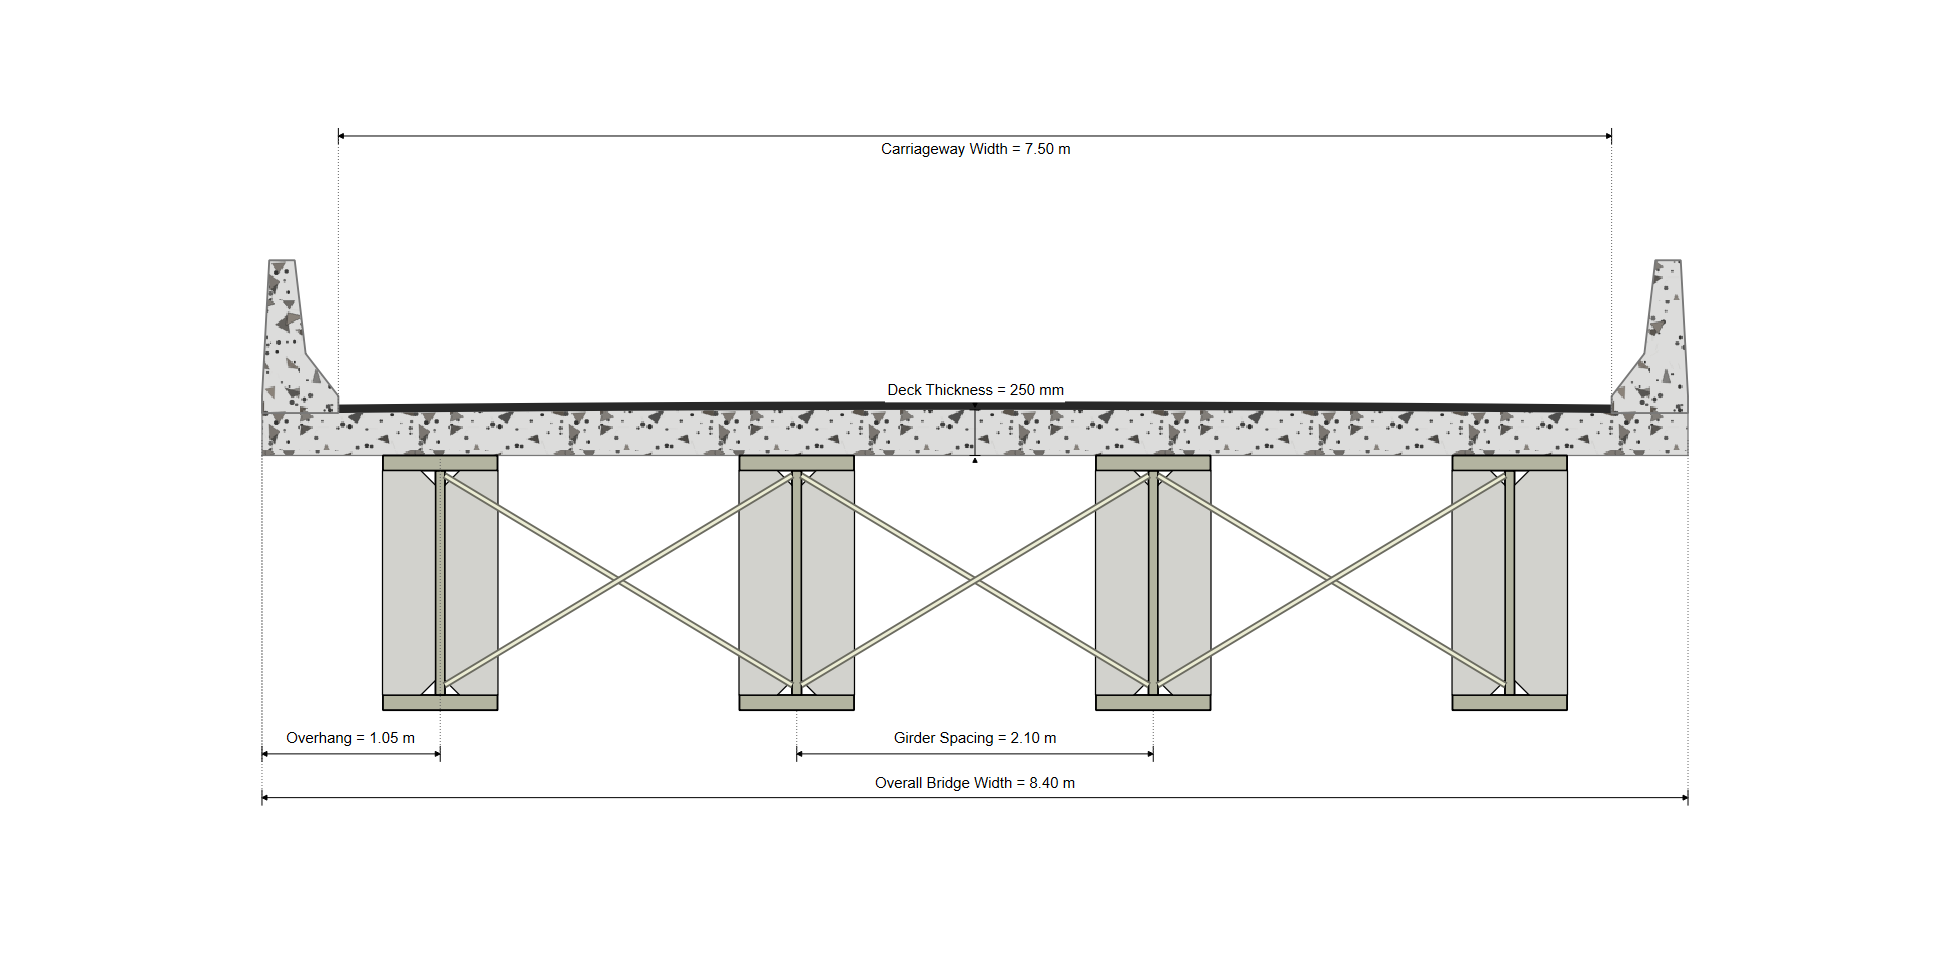
\includegraphics[width=\textwidth]{images/fig5_cad_cross_section.png}
        \caption{Transverse Cross-Section CAD View}
        \label{fig:cad_cross}
    \end{subfigure}
    \hfill
    \begin{subfigure}[b]{0.48\textwidth}
        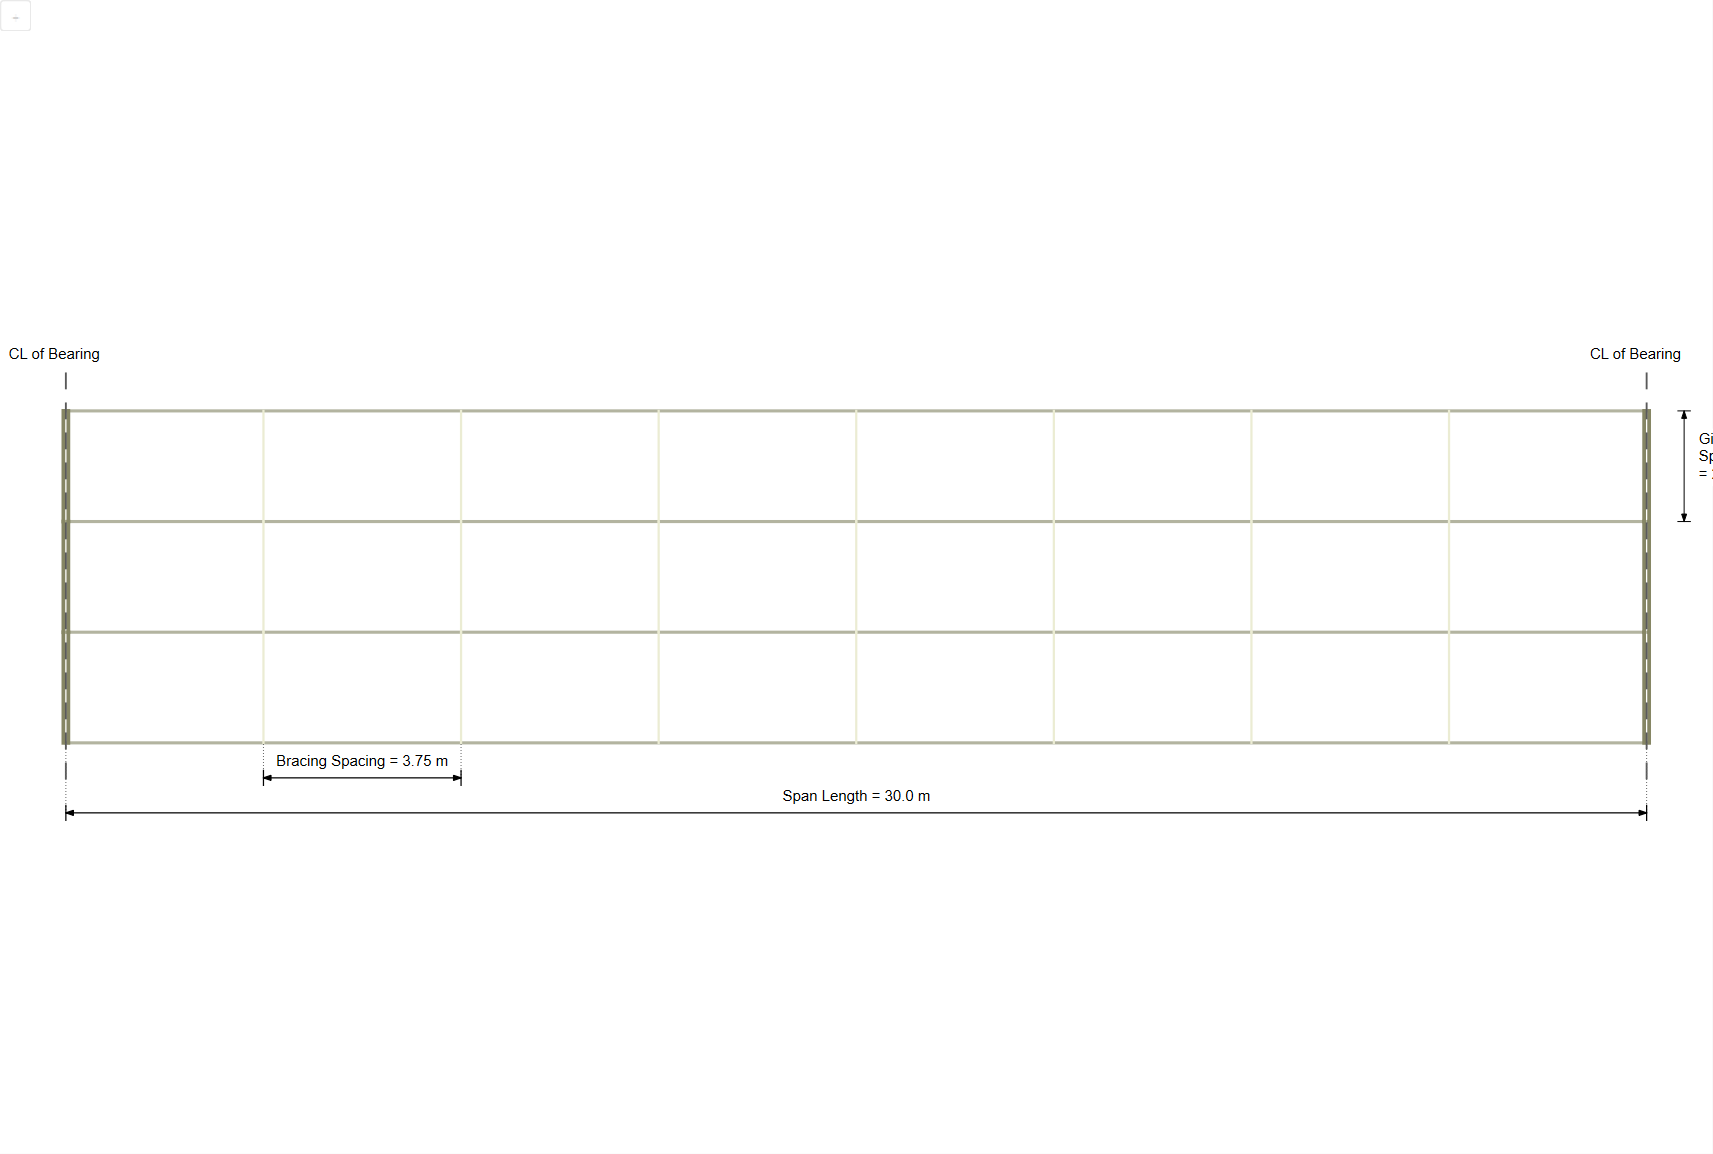
\includegraphics[width=\textwidth]{images/fig6_cad_top_view.png}
        \caption{Top Plan CAD View}
        \label{fig:cad_top}
    \end{subfigure}
    \caption{2D CAD Drafting Views Generated from Baseline Bridge Inputs (TC01)}
    \label{fig:cad_views}
\end{figure}

The transverse cross-section cleanly drafts the 4 plate girders, reinforced concrete deck slab, cantilever overhangs, crash barriers, and cross-frame spacing. The top view reflects the 30\,m span, girder alignment, and transverse diaphragm positions.

\subsection{3D OpenCASCADE Model Viewers and Input Dock}
Direct OpenGL framebuffer dumps (\texttt{ExportToImage}) were generated using OpenCASCADE's native offscreen pipeline:

\begin{figure}[H]
    \centering
    \begin{subfigure}[b]{0.48\textwidth}
        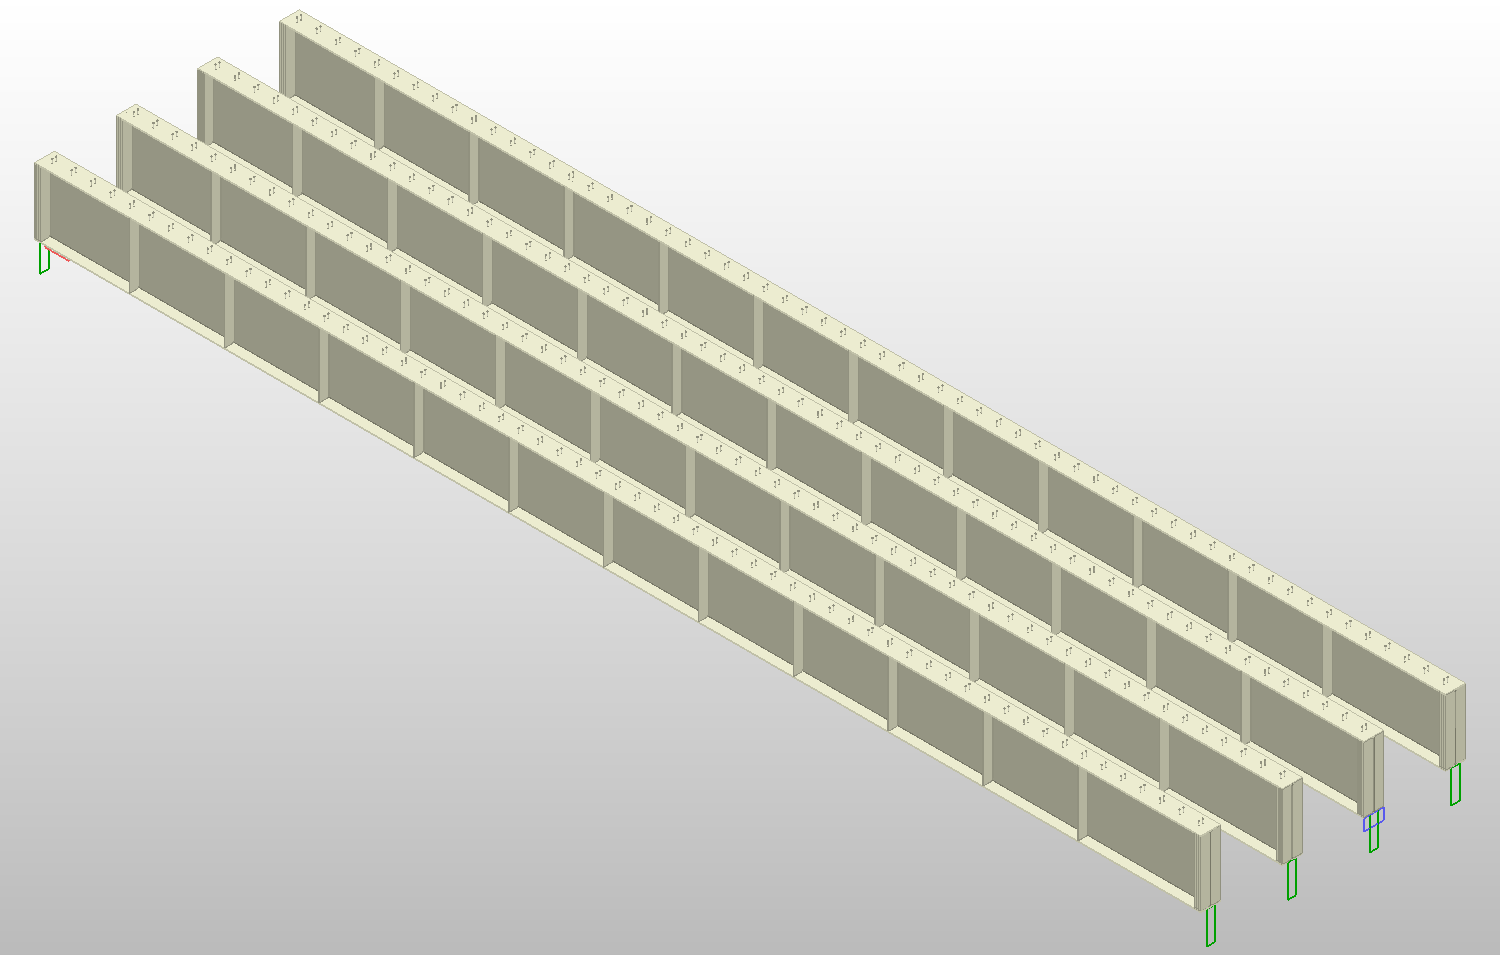
\includegraphics[width=\textwidth,height=4.6cm,keepaspectratio]{images/fig7_3d_girder_3d.png}
        \caption{Isometric View: Plate Girders \& Stiffeners}
        \label{fig:cad_3d_girder}
    \end{subfigure}
    \hfill
    \begin{subfigure}[b]{0.48\textwidth}
        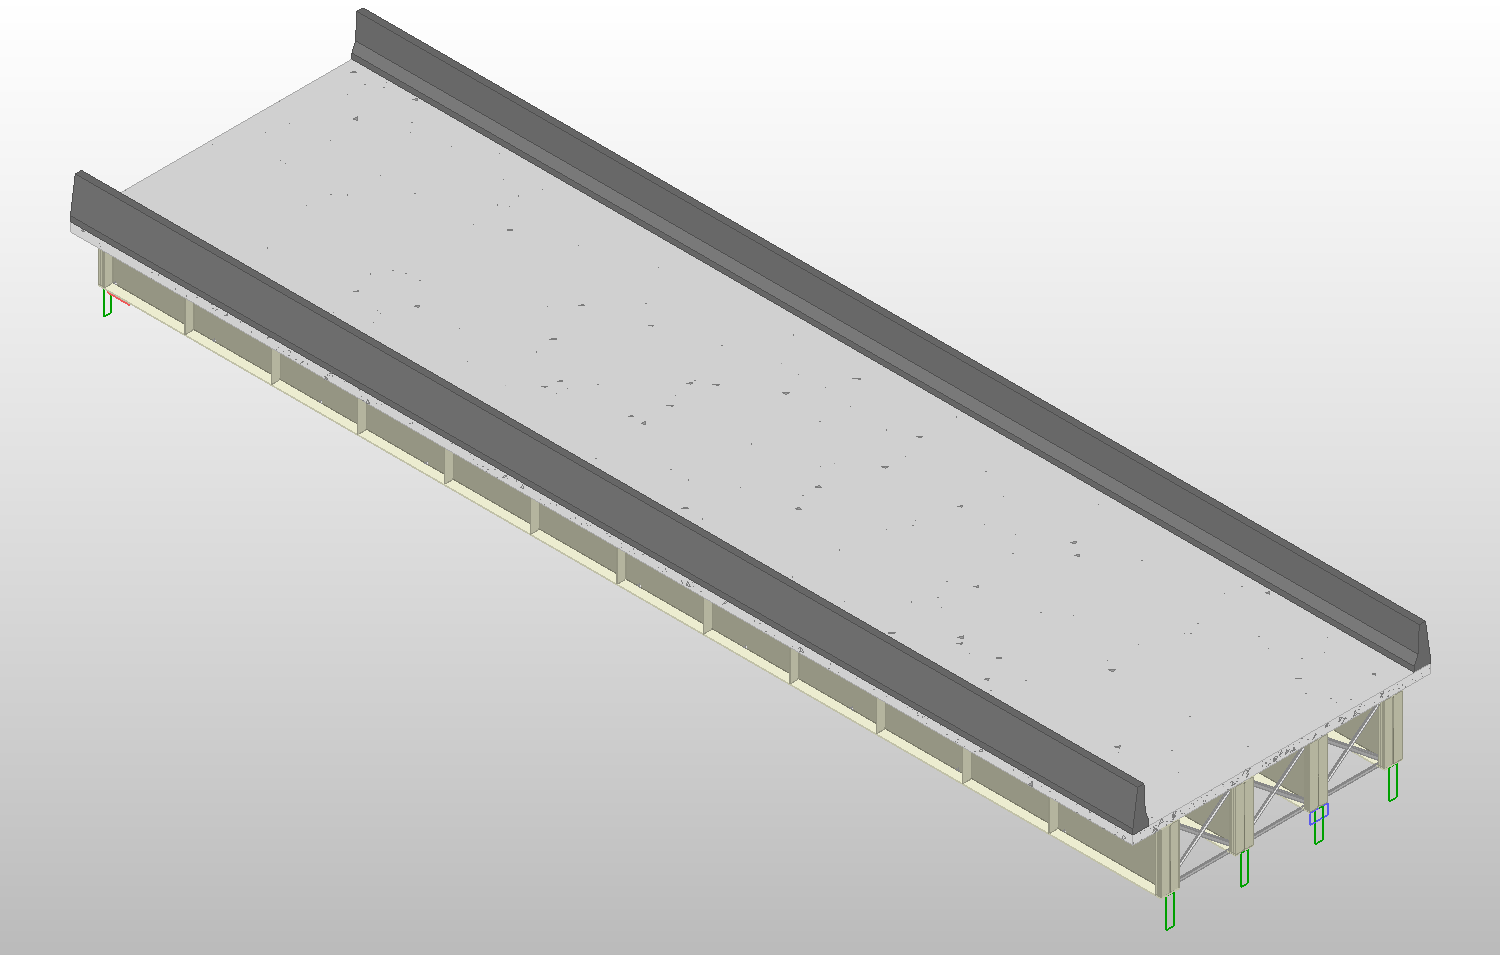
\includegraphics[width=\textwidth,height=4.6cm,keepaspectratio]{images/fig7_3d_final_geometry.png}
        \caption{Isometric View: Full Bridge Superstructure}
        \label{fig:cad_3d_full}
    \end{subfigure}
    \caption{OpenCASCADE 3D CAD Solid Model Renders (Direct OpenGL Framebuffer Export)}
    \label{fig:cad_3d_renders}
\end{figure}

\begin{figure}[H]
    \centering
    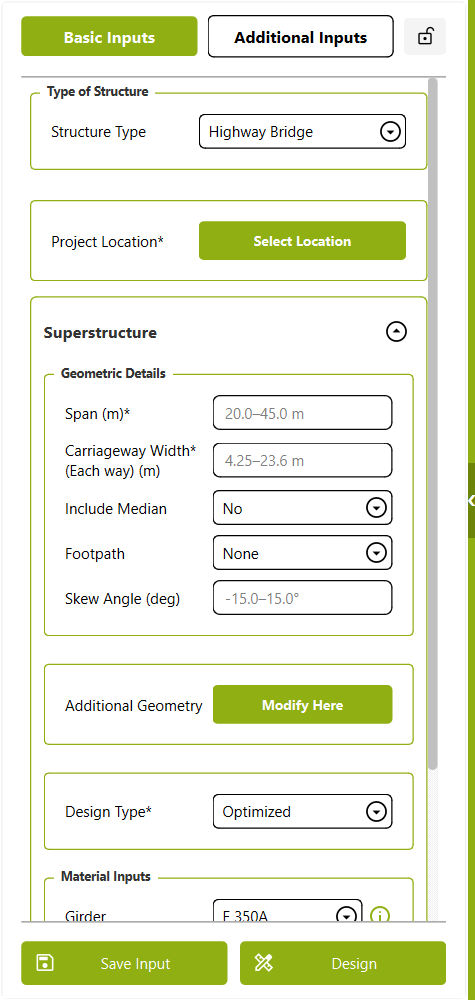
\includegraphics[width=0.38\textwidth,height=5.2cm,keepaspectratio]{images/fig4_input_dock_ui.png}
    \caption{OsdagBridge Desktop GUI: Input Dock Interface}
    \label{fig:input_dock}
\end{figure}

\subsection{UI Inspection Findings}
\begin{itemize}
    \item \textbf{Component Visibility}: Girders, stiffeners, cross-bracings, deck slabs, crash barriers, railings, and medians are cleanly toggleable via the 3D dock component checkboxes.
    \item \textbf{Identified Gap}: In \texttt{cad\_generator.py} (line 1050), key \texttt{KEY\_CAD\_END\_DIAPHRAGM} is missing from \texttt{hover\_dict} and \texttt{display\_3dModel()}, preventing users from isolating end diaphragms individually in the 3D viewer.
\end{itemize}

\newpage
\section{Formal GitHub Bug Reports and Code-Level Fixes}

\subsection{Issue 1: Concrete Deck Misclassification in MaterialPropertiesDialog}
\begin{tcolorbox}[colback=red!5!white,colframe=red!75!black,title=\textbf{Bug Summary: Deck Material Misclassified as Steel}]
\textbf{File}: \texttt{material\_properties.py} (lines 180, 435--438) \\
\textbf{Module}: \texttt{src/osdagbridge/desktop/ui/dialogs/} \\
\textbf{Impact}: Clicking info button on Deck Concrete Grade shows steel parameters ($F_y, F_u, G$) instead of concrete ($f_{ck}, f_{ctm}, E_{cm}$). Exporting leaves \texttt{material.deck.fck} unpopulated, causing \texttt{ValueError} in downstream design check.
\end{tcolorbox}

\begin{figure}[H]
    \centering
    \begin{subfigure}[b]{0.48\textwidth}
        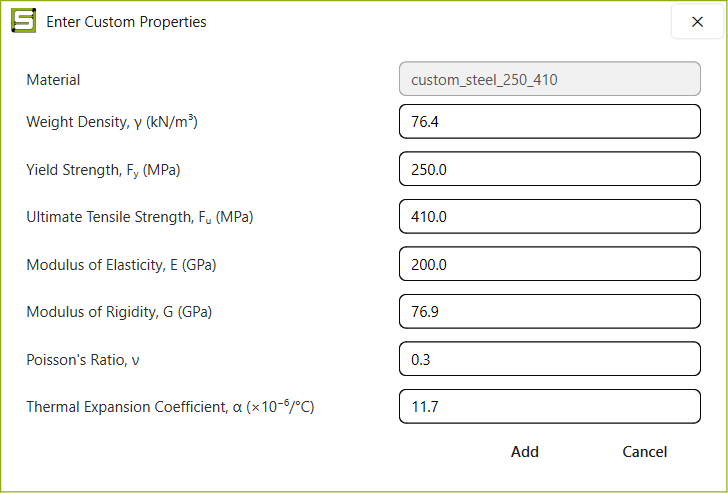
\includegraphics[width=\textwidth,height=3.8cm,keepaspectratio]{images/fig1_concrete_deck_misclassification_bug.png}
        \caption{Actual Bug: Concrete Deck Shown as Steel ($F_y, F_u$)}
        \label{fig:deck_bug}
    \end{subfigure}
    \hfill
    \begin{subfigure}[b]{0.48\textwidth}
        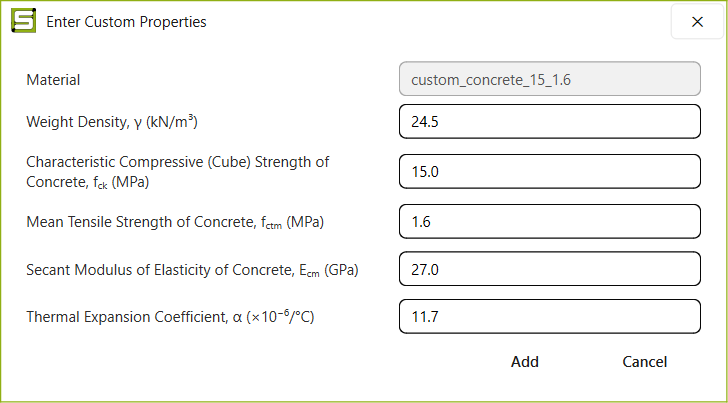
\includegraphics[width=\textwidth,height=3.8cm,keepaspectratio]{images/fig2_concrete_deck_dialog_expected.png}
        \caption{Expected: Concrete Properties ($f_{ck}, f_{ctm}, E_{cm}$)}
        \label{fig:deck_expected}
    \end{subfigure}
    \caption{Visual Evidence of Concrete Deck Misclassification in MaterialPropertiesDialog}
    \label{fig:dialog_comparison}
\end{figure}

\subsubsection*{Steps to Reproduce}
\begin{enumerate}
    \item In the Plate Girder Bridge window, view the \textbf{Deck Concrete Grade} field (e.g. \texttt{"M 35"}).
    \item Click the info button next to the combo box.
    \item Notice that the dialog displays structural steel properties (Yield Strength, Tensile Strength) rather than concrete compressive strength.
\end{enumerate}

\subsubsection*{Root Cause}
\texttt{InputDock} passes parameter \texttt{member="material.deck"}. However, \texttt{MaterialPropertiesDialog} only checks \texttt{self.member == "Deck"}. The fallback \texttt{\_is\_deck\_material("M 35")} fails because the SQLite database stores grades without spaces (\texttt{"M35"}). Thus, \texttt{self.is\_deck\_material} evaluates to \texttt{False}.

\subsubsection*{Proposed Code Fix}
\begin{lstlisting}
--- a/src/osdagbridge/desktop/ui/dialogs/material_properties.py
+++ b/src/osdagbridge/desktop/ui/dialogs/material_properties.py
@@ -180,2 +180,3 @@ class MaterialPropertiesDialog(QDialog):
-        self.is_deck_material = (self.member == "Deck") or self._is_deck_material(self.selected_material)
+        self.is_deck_material = (self.member in ("Deck", KEY_DECK_CONCRETE_GRADE_BASIC) or
+                                 self._is_deck_material(self.selected_material))
@@ -436,3 +437,3 @@ class MaterialPropertiesDialog(QDialog):
-        normalized = (material_name or "").strip()
-        return (normalized in concrete_properies or 
+        norm = (material_name or "").replace(" ", "").upper()
+        db_grades = [g.replace(" ", "").upper() for g in concrete_properies]
+        return (norm in db_grades or norm.lower().startswith(CUSTOM_CONCRETE_PREFIX))
\end{lstlisting}

\newpage
\subsection{Issue 2: Girder Dimension Corruption Across Consecutive Design Runs}
\begin{tcolorbox}[colback=red!5!white,colframe=red!75!black,title=\textbf{Bug Summary: Successive Unit Division Collapsing Section Geometry (Resolving Issue \#135)}]
\textbf{File}: \texttt{plategirderbridge.py} (lines 570--575, 680--685) \\
\textbf{Module}: \texttt{src/osdagbridge/core/bridge\_types/plate\_girder/} \\
\textbf{Impact}: Consecutive redesigns divide dimensions by 1000 on each run, shrinking depth to 1.67~mm and causing LTB calculation crash (\texttt{math domain error}).
\end{tcolorbox}

\subsubsection*{Steps to Reproduce}
\begin{enumerate}
    \item Run \texttt{design()} on a bridge instance with span 30\,m (girder depth 1670\,mm converted to 1.67\,m).
    \item Unlock the design and change an input that does not recalculate default depth (e.g. project location, skew angle, or custom sizing).
    \item Re-run \texttt{design()} on the same instance.
    \item Observe depth become 0.00167\,m (1.67\,mm), producing negative clear web depth and crashing LTB checks.
\end{enumerate}

\subsubsection*{Proposed Snapshot-and-Restore Implementation}
Downstream analysis and design routines access \texttt{self.input\_dict} in metres during solver execution. To preserve compatibility across downstream stages without mutating inputs across consecutive runs, we implement a \textbf{snapshot-and-restore contract} inside \texttt{PlateGirderBridge.design()}. This retains \texttt{self.input\_dict} in pristine UI millimetres between executions while guaranteeing downstream solvers receive metre values during computation:

\begin{lstlisting}
--- a/src/osdagbridge/core/bridge_types/plate_girder/plategirderbridge.py
+++ b/src/osdagbridge/core/bridge_types/plate_girder/plategirderbridge.py
@@ -570,6 +570,10 @@ class PlateGirderBridge:
         keys_to_convert = list(_DIM_KEYS_ALL_MODES)
         if not is_optimized:
             keys_to_convert.extend(_DIM_KEYS_NON_OPTIMIZED)
+        # Save pristine millimetre snapshot before in-place conversion
+        if not getattr(self, "_raw_ui_dims_mm", None):
+            self._raw_ui_dims_mm = {k: inp[k] for k in keys_to_convert if k in inp and inp[k] is not None}
@@ -680,4 +684,8 @@ class PlateGirderBridge:
         try:
+            # Restore pristine UI mm inputs before conversion on consecutive runs
+            if getattr(self, "_raw_ui_dims_mm", None):
+                for k, mm_val in self._raw_ui_dims_mm.items():
+                    if k in self.input_dict and isinstance(self.input_dict[k], (int, float)) and self.input_dict[k] < 10.0:
+                        self.input_dict[k] = mm_val
             self._resolve_optimized_bounds_to_mm()
             self._convert_girder_dims_mm_to_m()
\end{lstlisting}

\subsubsection*{Regression Verification and Results}
An isolated multi-run regression test was executed on an active \texttt{PlateGirderBridge} model instance to verify this contract across three sequential executions without re-priming from defaults. On each run, girder depth was restored to 1670.0\,mm and converted to 1.670\,m (Run 1: 1.670\,m, Run 2: 1.670\,m, Run 3: 1.670\,m; all PASS). Clear web depth remained positive ($d_{web} = 1.626\text{ m}$), eliminating the negative radicand in $M_{cr}$ and verifying that this contract completely resolves GitHub Issue \#135.

\newpage
\subsection{Issue 3: Custom Material Density Bypass in Analysis Dead Loads}
\begin{tcolorbox}[colback=red!5!white,colframe=red!75!black,title=\textbf{Bug Summary: Dead Load Pipeline Ignores Custom Densities}]
\textbf{Files}: \texttt{plategirderbridge.py:1192, 1333} and \texttt{analyser.py:416} \\
\textbf{Module}: \texttt{src/osdagbridge/core/bridge\_types/plate\_girder/} \\
\textbf{Impact}: Dead loads and reactions ignore user-defined steel and concrete densities, hardcoding $78.5\text{ kN/m}^3$ and $25.0\text{ kN/m}^3$.
\end{tcolorbox}

\subsubsection*{Proposed Multi-Module Patch (Architectural Forwarding)}
While user-specified modulus and strength values are forwarded to design checks, dead load calculations bypass custom densities. The following proposed patch outlines the multi-module changes required to route custom steel and concrete densities through to the dead load generator in \texttt{analyser.py}:

\begin{lstlisting}
--- a/src/osdagbridge/core/bridge_types/plate_girder/plategirderbridge.py
+++ b/src/osdagbridge/core/bridge_types/plate_girder/plategirderbridge.py
@@ -1193,2 +1193,4 @@ class PlateGirderBridge:
         if rho is None:
-            rho = _DEFAULT_DENSITY
+            raw_rho = self.input_dict.get(KEY_MATERIAL_GIRDER_DENSITY)
+            rho = float(raw_rho) * 1000.0 if raw_rho not in (None, "") else _DEFAULT_DENSITY
@@ -1333,2 +1335,4 @@ class PlateGirderBridge:
-        model.create_deck_load(slab_thickness_m=deck_t_m)
+        deck_density = float(self.input_dict.get(KEY_MATERIAL_DECK_DENSITY, 25.0))
+        model.create_deck_load(slab_thickness_m=deck_t_m, concrete_density_kN_m3=deck_density)

--- a/src/osdagbridge/core/bridge_types/plate_girder/analyser.py
+++ b/src/osdagbridge/core/bridge_types/plate_girder/analyser.py
@@ -413,4 +413,6 @@ class GrillageModel:
+        steel_rho = (self.material_props.steel.rho / 1000.0) if hasattr(self, 'material_props') and self.material_props else STEEL_UNIT_WEIGHT_kN_m3
         for z_pos in model.Mesh_obj.noz[1:-1]:
             A_girder_m2 = _area_for_z(z_pos)
-            beam_mag = girder_self_weight_kN_m(A_girder_m2, STEEL_UNIT_WEIGHT_kN_m3) * kN / m
+            beam_mag = girder_self_weight_kN_m(A_girder_m2, steel_rho) * kN / m
\end{lstlisting}

\subsubsection*{Recommended Regression Verification}
To validate this patch before integration into production, we recommend adding an automated regression test comparing dead load reactions with default vs.\ custom densities ($\rho_{steel} = 80.0\text{ kN/m}^3$, $\rho_{conc} = 26.0\text{ kN/m}^3$). Support reactions and dead load bending moments in \texttt{model.dataset} should scale proportionally ($\approx +1.9\%$ for steel self-weight, $+4.0\%$ for deck dead load).

\newpage
\section{Recommendations and Conclusions}

\subsection{Engineering Recommendations}
\begin{enumerate}
    \item \textbf{Prevent Input Data Mutation}: Formalize the snapshot-and-restore contract or transition to an immutable \texttt{AnalysisContext} object, ensuring UI units remain in millimetres between executions.
    \item \textbf{Consistent Unit and Material Handling}: Centralize material grade lookups to strip whitespace and normalize case before querying database tables.
    \item \textbf{Complete Dead Load Forwarding}: Integrate density properties into all self-weight and superimposed dead load functions in \texttt{analyser.py}.
    \item \textbf{Regression Testing}: Introduce regression unit tests covering consecutive redesign calls on unlocked models, verifying that dimensional keys retain consistent values across runs.
\end{enumerate}

\subsection{Conclusion}
This study evaluated OsdagBridge's short-span steel plate girder module as part of the FOSSEE Winter Internship screening task. Eight test scenarios covering geometric boundaries, skew angles, custom materials, and repeated design runs were executed and documented. 

The testing verified the end-to-end design pipeline while distinguishing software execution success from structural design check verdicts (where initial trial sections govern in fatigue). Crucially, the testing identified three code-level issues—including isolating the exact root cause of the second-run crash previously noted in GitHub Issue \#135. Actionable code patches, verified snapshot-and-restore regression tests for Issue \#135, and recommended integration verification criteria have been provided for each issue. These findings support further improvements to OsdagBridge's reliability, stability, and adherence to structural design codes.

\end{document}
